\documentclass[1p]{elsarticle_modified}
%\bibliographystyle{elsarticle-num}

%\usepackage[colorlinks]{hyperref}
%\usepackage{abbrmath_seonhwa} %\Abb, \Ascr, \Acal ,\Abf, \Afrak
\usepackage{amsfonts}
\usepackage{amssymb}
\usepackage{amsmath}
\usepackage{amsthm}
\usepackage{scalefnt}
\usepackage{amsbsy}
\usepackage{kotex}
\usepackage{caption}
\usepackage{subfig}
\usepackage{color}
\usepackage{graphicx}
\usepackage{xcolor} %% white, black, red, green, blue, cyan, magenta, yellow
\usepackage{float}
\usepackage{setspace}
\usepackage{hyperref}

\usepackage{tikz}
\usetikzlibrary{arrows}

\usepackage{multirow}
\usepackage{array} % fixed length table
\usepackage{hhline}

%%%%%%%%%%%%%%%%%%%%%
\makeatletter
\renewcommand*\env@matrix[1][\arraystretch]{%
	\edef\arraystretch{#1}%
	\hskip -\arraycolsep
	\let\@ifnextchar\new@ifnextchar
	\array{*\c@MaxMatrixCols c}}
\makeatother %https://tex.stackexchange.com/questions/14071/how-can-i-increase-the-line-spacing-in-a-matrix
%%%%%%%%%%%%%%%

\usepackage[normalem]{ulem}

\newcommand{\msout}[1]{\ifmmode\text{\sout{\ensuremath{#1}}}\else\sout{#1}\fi}
%SOURCE: \msout is \stkout macro in https://tex.stackexchange.com/questions/20609/strikeout-in-math-mode

\newcommand{\cancel}[1]{
	\ifmmode
	{\color{red}\msout{#1}}
	\else
	{\color{red}\sout{#1}}
	\fi
}

\newcommand{\add}[1]{
	{\color{blue}\uwave{#1}}
}

\newcommand{\replace}[2]{
	\ifmmode
	{\color{red}\msout{#1}}{\color{blue}\uwave{#2}}
	\else
	{\color{red}\sout{#1}}{\color{blue}\uwave{#2}}
	\fi
}

\newcommand{\Sol}{\mathcal{S}} %segment
\newcommand{\D}{D} %diagram
\newcommand{\A}{\mathcal{A}} %arc


%%%%%%%%%%%%%%%%%%%%%%%%%%%%%5 test

\def\sl{\operatorname{\textup{SL}}(2,\Cbb)}
\def\psl{\operatorname{\textup{PSL}}(2,\Cbb)}
\def\quan{\mkern 1mu \triangleright \mkern 1mu}

\theoremstyle{definition}
\newtheorem{thm}{Theorem}[section]
\newtheorem{prop}[thm]{Proposition}
\newtheorem{lem}[thm]{Lemma}
\newtheorem{ques}[thm]{Question}
\newtheorem{cor}[thm]{Corollary}
\newtheorem{defn}[thm]{Definition}
\newtheorem{exam}[thm]{Example}
\newtheorem{rmk}[thm]{Remark}
\newtheorem{alg}[thm]{Algorithm}

\newcommand{\I}{\sqrt{-1}}
\begin{document}

%\begin{frontmatter}
%
%\title{Boundary parabolic representations of knots up to 8 crossings}
%
%%% Group authors per affiliation:
%\author{Yunhi Cho} 
%\address{Department of Mathematics, University of Seoul, Seoul, Korea}
%\ead{yhcho@uos.ac.kr}
%
%
%\author{Seonhwa Kim} %\fnref{s_kim}}
%\address{Center for Geometry and Physics, Institute for Basic Science, Pohang, 37673, Korea}
%\ead{ryeona17@ibs.re.kr}
%
%\author{Hyuk Kim}
%\address{Department of Mathematical Sciences, Seoul National University, Seoul 08826, Korea}
%\ead{hyukkim@snu.ac.kr}
%
%\author{Seokbeom Yoon}
%\address{Department of Mathematical Sciences, Seoul National University, Seoul, 08826,  Korea}
%\ead{sbyoon15@snu.ac.kr}
%
%\begin{abstract}
%We find all boundary parabolic representation of knots up to 8 crossings.
%
%\end{abstract}
%\begin{keyword}
%    \MSC[2010] 57M25 
%\end{keyword}
%
%\end{frontmatter}

%\linenumbers
%\tableofcontents
%
\newcommand\colored[1]{\textcolor{white}{\rule[-0.35ex]{0.8em}{1.4ex}}\kern-0.8em\color{red} #1}%
%\newcommand\colored[1]{\textcolor{white}{ #1}\kern-2.17ex	\textcolor{white}{ #1}\kern-1.81ex	\textcolor{white}{ #1}\kern-2.15ex\color{red}#1	}

{\Large $\underline{12a_{0216}~(K12a_{0216})}$}

\setlength{\tabcolsep}{10pt}
\renewcommand{\arraystretch}{1.6}
\vspace{1cm}\begin{tabular}{m{100pt}>{\centering\arraybackslash}m{274pt}}
\multirow{5}{120pt}{
	\centering
	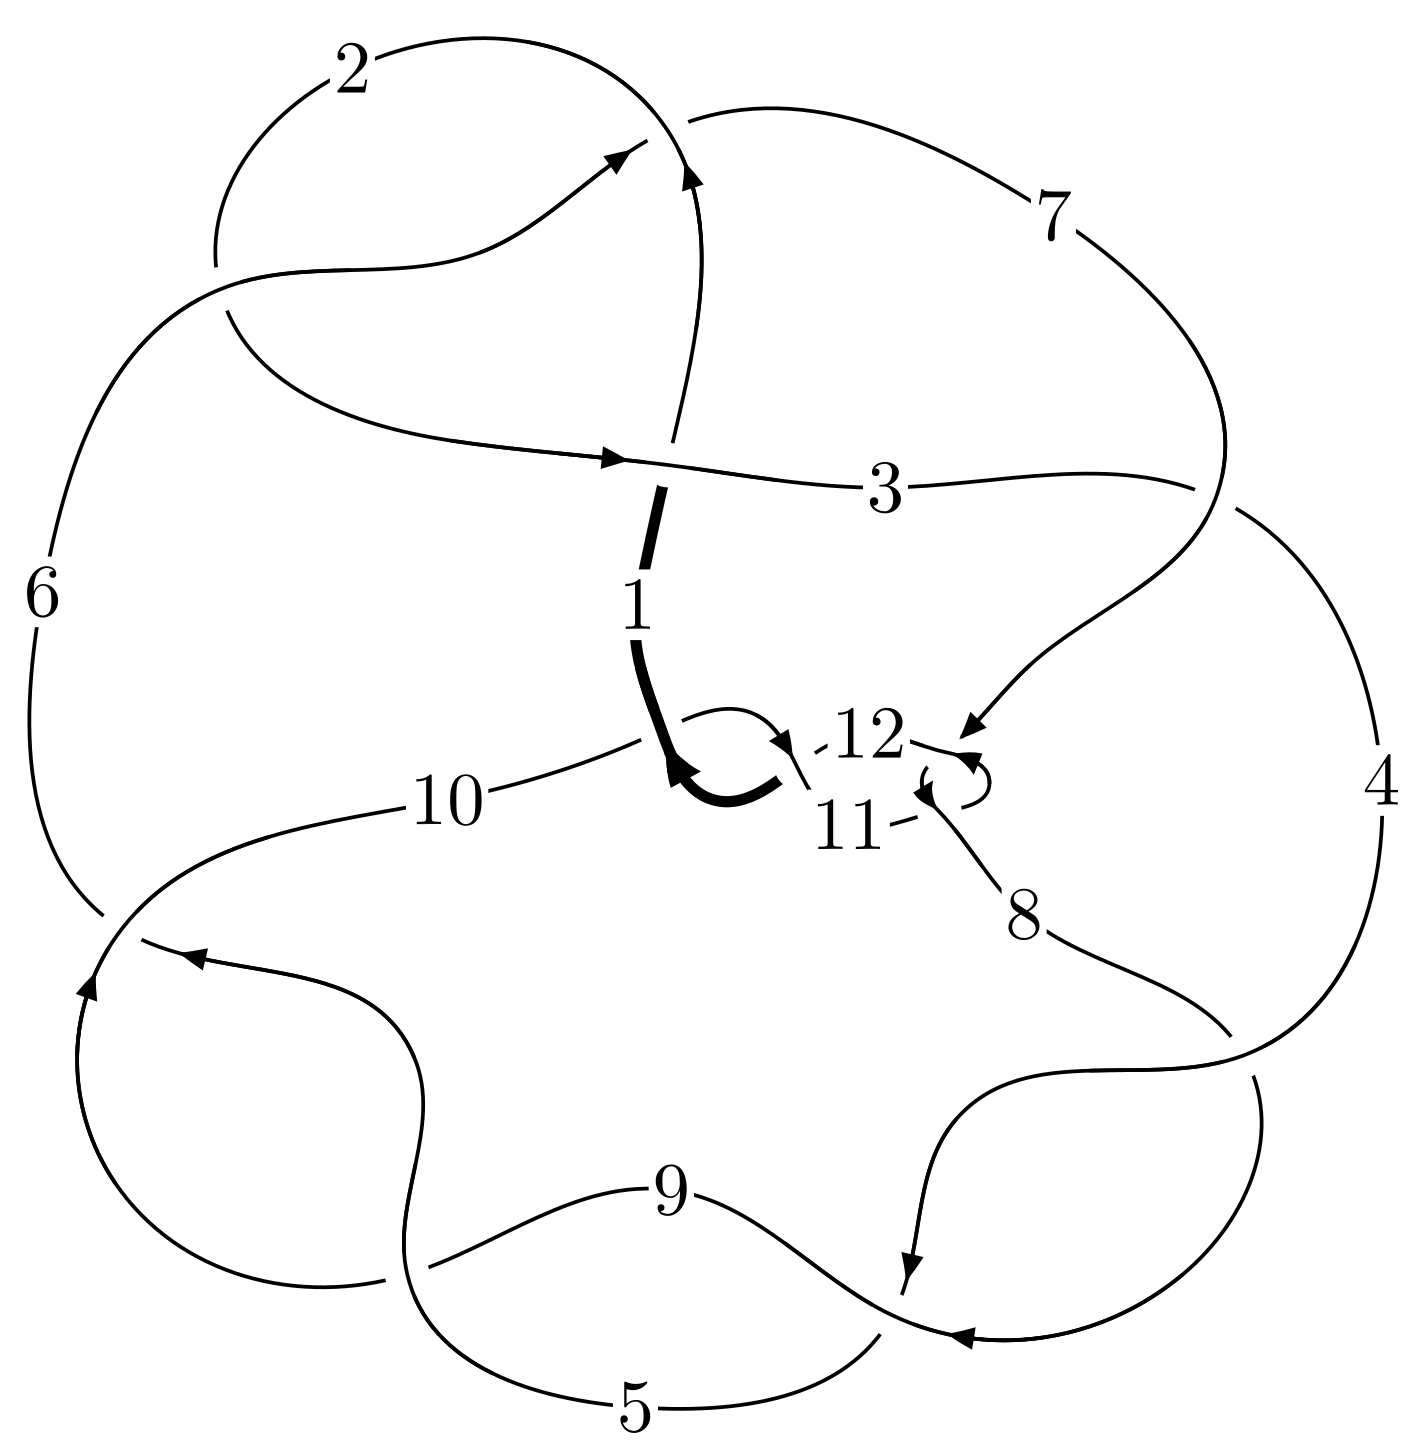
\includegraphics[width=112pt]{../../../GIT/diagram.site/Diagrams/png/1017_12a_0216.png}\\
\ \ \ A knot diagram\footnotemark}&
\allowdisplaybreaks
\textbf{Linearized knot diagam} \\
\cline{2-2}
 &
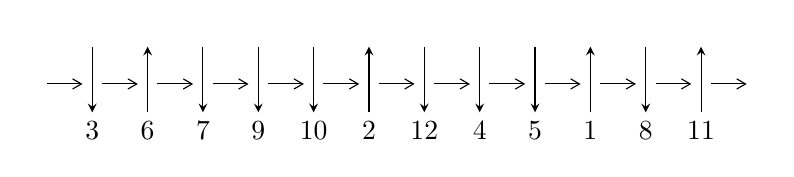
\begin{tikzpicture}[x=20pt, y=17pt]
	% nodes
	\node (C0) at (0, 0) {};
	\node (C1) at (1, 0) {};
	\node (C1U) at (1, +1) {};
	\node (C1D) at (1, -1) {3};

	\node (C2) at (2, 0) {};
	\node (C2U) at (2, +1) {};
	\node (C2D) at (2, -1) {6};

	\node (C3) at (3, 0) {};
	\node (C3U) at (3, +1) {};
	\node (C3D) at (3, -1) {7};

	\node (C4) at (4, 0) {};
	\node (C4U) at (4, +1) {};
	\node (C4D) at (4, -1) {9};

	\node (C5) at (5, 0) {};
	\node (C5U) at (5, +1) {};
	\node (C5D) at (5, -1) {10};

	\node (C6) at (6, 0) {};
	\node (C6U) at (6, +1) {};
	\node (C6D) at (6, -1) {2};

	\node (C7) at (7, 0) {};
	\node (C7U) at (7, +1) {};
	\node (C7D) at (7, -1) {12};

	\node (C8) at (8, 0) {};
	\node (C8U) at (8, +1) {};
	\node (C8D) at (8, -1) {4};

	\node (C9) at (9, 0) {};
	\node (C9U) at (9, +1) {};
	\node (C9D) at (9, -1) {5};

	\node (C10) at (10, 0) {};
	\node (C10U) at (10, +1) {};
	\node (C10D) at (10, -1) {1};

	\node (C11) at (11, 0) {};
	\node (C11U) at (11, +1) {};
	\node (C11D) at (11, -1) {8};

	\node (C12) at (12, 0) {};
	\node (C12U) at (12, +1) {};
	\node (C12D) at (12, -1) {11};
	\node (C13) at (13, 0) {};

	% arrows
	\draw[->,>={angle 60}]
	(C0) edge (C1) (C1) edge (C2) (C2) edge (C3) (C3) edge (C4) (C4) edge (C5) (C5) edge (C6) (C6) edge (C7) (C7) edge (C8) (C8) edge (C9) (C9) edge (C10) (C10) edge (C11) (C11) edge (C12) (C12) edge (C13) ;	\draw[->,>=stealth]
	(C1U) edge (C1D) (C2D) edge (C2U) (C3U) edge (C3D) (C4U) edge (C4D) (C5U) edge (C5D) (C6D) edge (C6U) (C7U) edge (C7D) (C8U) edge (C8D) (C9U) edge (C9D) (C10D) edge (C10U) (C11U) edge (C11D) (C12D) edge (C12U) ;
	\end{tikzpicture} \\
\hhline{~~} \\& 
\textbf{Solving Sequence} \\ \cline{2-2} 
 &
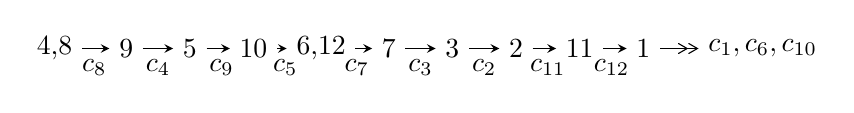
\begin{tikzpicture}[x=23pt, y=7pt]
	% node
	\node (A0) at (-1/8, 0) {4,8};
	\node (A1) at (1, 0) {9};
	\node (A2) at (2, 0) {5};
	\node (A3) at (3, 0) {10};
	\node (A4) at (65/16, 0) {6,12};
	\node (A5) at (41/8, 0) {7};
	\node (A6) at (49/8, 0) {3};
	\node (A7) at (57/8, 0) {2};
	\node (A8) at (65/8, 0) {11};
	\node (A9) at (73/8, 0) {1};
	\node (C1) at (1/2, -1) {$c_{8}$};
	\node (C2) at (3/2, -1) {$c_{4}$};
	\node (C3) at (5/2, -1) {$c_{9}$};
	\node (C4) at (7/2, -1) {$c_{5}$};
	\node (C5) at (37/8, -1) {$c_{7}$};
	\node (C6) at (45/8, -1) {$c_{3}$};
	\node (C7) at (53/8, -1) {$c_{2}$};
	\node (C8) at (61/8, -1) {$c_{11}$};
	\node (C9) at (69/8, -1) {$c_{12}$};
	\node (A10) at (11, 0) {$c_{1},c_{6},c_{10}$};

	% edge
	\draw[->,>=stealth]	
	(A0) edge (A1) (A1) edge (A2) (A2) edge (A3) (A3) edge (A4) (A4) edge (A5) (A5) edge (A6) (A6) edge (A7) (A7) edge (A8) (A8) edge (A9) ;
	\draw[->>,>={angle 60}]	
	(A9) edge (A10);
\end{tikzpicture} \\ 

\end{tabular} \\

\footnotetext{
The image of knot diagram is generated by the software ``\textbf{Draw programme}" developed by Andrew Bartholomew(\url{http://www.layer8.co.uk/maths/draw/index.htm\#Running-draw}), where we modified some parts for our purpose(\url{https://github.com/CATsTAILs/LinksPainter}).
}\phantom \\ \newline 
\centering \textbf{Ideals for irreducible components\footnotemark of $X_{\text{par}}$} 
 
\begin{align*}
I^u_{1}&=\langle 
3.31230\times10^{33} u^{63}-9.21845\times10^{33} u^{62}+\cdots+2.52277\times10^{34} b-5.95857\times10^{34},\\
\phantom{I^u_{1}}&\phantom{= \langle  }1.05553\times10^{34} u^{63}-2.85080\times10^{34} u^{62}+\cdots+2.52277\times10^{34} a-9.65444\times10^{33},\;u^{64}-4 u^{63}+\cdots+32 u+16\rangle \\
I^u_{2}&=\langle 
2 b+2 a- u+2,\;2 a^2-2 a u+2 a- u+3,\;u^2-2\rangle \\
I^u_{3}&=\langle 
a^4 u-2 a^4+4 a^3 u-8 a^3+4 a^2 u-8 a^2-7 a u+25 b-11 a-14 u-2,\\
\phantom{I^u_{3}}&\phantom{= \langle  }a^5+2 a^4 u+2 a^4+3 a^3 u+6 a^3+8 a^2 u+10 a^2+7 a u+13 a- u-1,\;u^2+u-1\rangle \\
I^u_{4}&=\langle 
a u+b+2 a+u+2,\;2 a^2+a u+2 a- u+3,\;u^2-2\rangle \\
\\
I^v_{1}&=\langle 
a,\;b- v-1,\;v^2+v+1\rangle \\
I^v_{2}&=\langle 
a,\;b^2- b+1,\;v-1\rangle \\
\end{align*}
\raggedright * 6 irreducible components of $\dim_{\mathbb{C}}=0$, with total 86 representations.\\
\footnotetext{All coefficients of polynomials are rational numbers. But the coefficients are sometimes approximated in decimal forms when there is not enough margin.}
\newpage
\renewcommand{\arraystretch}{1}
\centering \section*{I. $I^u_{1}= \langle 3.31\times10^{33} u^{63}-9.22\times10^{33} u^{62}+\cdots+2.52\times10^{34} b-5.96\times10^{34},\;1.06\times10^{34} u^{63}-2.85\times10^{34} u^{62}+\cdots+2.52\times10^{34} a-9.65\times10^{33},\;u^{64}-4 u^{63}+\cdots+32 u+16 \rangle$}
\flushleft \textbf{(i) Arc colorings}\\
\begin{tabular}{m{7pt} m{180pt} m{7pt} m{180pt} }
\flushright $a_{4}=$&$\begin{pmatrix}0\\u\end{pmatrix}$ \\
\flushright $a_{8}=$&$\begin{pmatrix}1\\0\end{pmatrix}$ \\
\flushright $a_{9}=$&$\begin{pmatrix}1\\u^2\end{pmatrix}$ \\
\flushright $a_{5}=$&$\begin{pmatrix}- u\\- u^3+u\end{pmatrix}$ \\
\flushright $a_{10}=$&$\begin{pmatrix}- u^2+1\\- u^4+2 u^2\end{pmatrix}$ \\
\flushright $a_{6}=$&$\begin{pmatrix}u^3-2 u\\u^5-3 u^3+u\end{pmatrix}$ \\
\flushright $a_{12}=$&$\begin{pmatrix}-0.418403 u^{63}+1.13003 u^{62}+\cdots+7.82001 u+0.382692\\-0.131296 u^{63}+0.365410 u^{62}+\cdots+4.28462 u+2.36192\end{pmatrix}$ \\
\flushright $a_{7}=$&$\begin{pmatrix}-0.342599 u^{63}+0.737839 u^{62}+\cdots+11.5782 u+4.46198\\-0.263432 u^{63}+0.630688 u^{62}+\cdots+6.03905 u+1.99604\end{pmatrix}$ \\
\flushright $a_{3}=$&$\begin{pmatrix}0.790350 u^{63}-2.05902 u^{62}+\cdots-18.5463 u-5.88736\\0.362768 u^{63}-0.965419 u^{62}+\cdots-6.85471 u-2.61286\end{pmatrix}$ \\
\flushright $a_{2}=$&$\begin{pmatrix}0.203141 u^{63}-0.562340 u^{62}+\cdots-3.81650 u-1.43156\\0.409877 u^{63}-1.08413 u^{62}+\cdots-8.12806 u-2.97524\end{pmatrix}$ \\
\flushright $a_{11}=$&$\begin{pmatrix}-0.549700 u^{63}+1.49544 u^{62}+\cdots+12.1046 u+2.74461\\-0.131296 u^{63}+0.365410 u^{62}+\cdots+4.28462 u+2.36192\end{pmatrix}$ \\
\flushright $a_{1}=$&$\begin{pmatrix}0.768798 u^{63}-1.82001 u^{62}+\cdots-19.8193 u-8.43548\\0.735613 u^{63}-1.86045 u^{62}+\cdots-15.0301 u-5.18940\end{pmatrix}$\\&\end{tabular}
\flushleft \textbf{(ii) Obstruction class $= -1$}\\~\\
\flushleft \textbf{(iii) Cusp Shapes $= 2.52449 u^{63}-5.73943 u^{62}+\cdots-69.7334 u-34.4634$}\\~\\
\newpage\renewcommand{\arraystretch}{1}
\flushleft \textbf{(iv) u-Polynomials at the component}\newline \\
\begin{tabular}{m{50pt}|m{274pt}}
Crossings & \hspace{64pt}u-Polynomials at each crossing \\
\hline $$\begin{aligned}c_{1}\end{aligned}$$&$\begin{aligned}
&u^{64}+35 u^{63}+\cdots+416 u+49
\end{aligned}$\\
\hline $$\begin{aligned}c_{2},c_{6}\end{aligned}$$&$\begin{aligned}
&u^{64}-3 u^{63}+\cdots-16 u+7
\end{aligned}$\\
\hline $$\begin{aligned}c_{3}\end{aligned}$$&$\begin{aligned}
&u^{64}+3 u^{63}+\cdots-4558 u+763
\end{aligned}$\\
\hline $$\begin{aligned}c_{4},c_{5},c_{8}\\c_{9}\end{aligned}$$&$\begin{aligned}
&u^{64}+4 u^{63}+\cdots-32 u+16
\end{aligned}$\\
\hline $$\begin{aligned}c_{7},c_{11}\end{aligned}$$&$\begin{aligned}
&u^{64}+3 u^{63}+\cdots-6 u+7
\end{aligned}$\\
\hline $$\begin{aligned}c_{10},c_{12}\end{aligned}$$&$\begin{aligned}
&u^{64}-19 u^{63}+\cdots-608 u+49
\end{aligned}$\\
\hline
\end{tabular}\\~\\
\newpage\renewcommand{\arraystretch}{1}
\flushleft \textbf{(v) Riley Polynomials at the component}\newline \\
\begin{tabular}{m{50pt}|m{274pt}}
Crossings & \hspace{64pt}Riley Polynomials at each crossing \\
\hline $$\begin{aligned}c_{1}\end{aligned}$$&$\begin{aligned}
&y^{64}-5 y^{63}+\cdots-30760 y+2401
\end{aligned}$\\
\hline $$\begin{aligned}c_{2},c_{6}\end{aligned}$$&$\begin{aligned}
&y^{64}+35 y^{63}+\cdots+416 y+49
\end{aligned}$\\
\hline $$\begin{aligned}c_{3}\end{aligned}$$&$\begin{aligned}
&y^{64}-45 y^{63}+\cdots+15204664 y+582169
\end{aligned}$\\
\hline $$\begin{aligned}c_{4},c_{5},c_{8}\\c_{9}\end{aligned}$$&$\begin{aligned}
&y^{64}-76 y^{63}+\cdots-1024 y+256
\end{aligned}$\\
\hline $$\begin{aligned}c_{7},c_{11}\end{aligned}$$&$\begin{aligned}
&y^{64}+19 y^{63}+\cdots+608 y+49
\end{aligned}$\\
\hline $$\begin{aligned}c_{10},c_{12}\end{aligned}$$&$\begin{aligned}
&y^{64}+59 y^{63}+\cdots+133272 y+2401
\end{aligned}$\\
\hline
\end{tabular}\\~\\
\newpage\flushleft \textbf{(vi) Complex Volumes and Cusp Shapes}
$$\begin{array}{c|c|c}  
\text{Solutions to }I^u_{1}& \I (\text{vol} + \sqrt{-1}CS) & \text{Cusp shape}\\
 \hline 
\begin{aligned}
u &= \phantom{-}0.873442 + 0.450062 I \\
a &= \phantom{-}0.316313 + 0.070275 I \\
b &= -0.799432 + 0.773699 I\end{aligned}
 & -4.38307 - 0.99571 I & \phantom{-0.000000 } 0 \\ \hline\begin{aligned}
u &= \phantom{-}0.873442 - 0.450062 I \\
a &= \phantom{-}0.316313 - 0.070275 I \\
b &= -0.799432 - 0.773699 I\end{aligned}
 & -4.38307 + 0.99571 I & \phantom{-0.000000 } 0 \\ \hline\begin{aligned}
u &= -0.819111 + 0.526710 I \\
a &= -1.11929 - 1.64147 I \\
b &= -0.751905 + 0.969822 I\end{aligned}
 & -3.78557 + 6.83757 I & \phantom{-0.000000 } 0 \\ \hline\begin{aligned}
u &= -0.819111 - 0.526710 I \\
a &= -1.11929 + 1.64147 I \\
b &= -0.751905 - 0.969822 I\end{aligned}
 & -3.78557 - 6.83757 I & \phantom{-0.000000 } 0 \\ \hline\begin{aligned}
u &= \phantom{-}0.824871 + 0.622233 I \\
a &= -0.92431 + 1.81972 I \\
b &= -0.773002 - 1.004690 I\end{aligned}
 & -6.66344 - 11.86030 I & \phantom{-0.000000 } 0 \\ \hline\begin{aligned}
u &= \phantom{-}0.824871 - 0.622233 I \\
a &= -0.92431 - 1.81972 I \\
b &= -0.773002 + 1.004690 I\end{aligned}
 & -6.66344 + 11.86030 I & \phantom{-0.000000 } 0 \\ \hline\begin{aligned}
u &= -0.879555 + 0.575858 I \\
a &= \phantom{-}0.533241 + 0.042734 I \\
b &= -0.858792 - 0.753406 I\end{aligned}
 & -7.43975 + 5.78092 I & \phantom{-0.000000 } 0 \\ \hline\begin{aligned}
u &= -0.879555 - 0.575858 I \\
a &= \phantom{-}0.533241 - 0.042734 I \\
b &= -0.858792 + 0.753406 I\end{aligned}
 & -7.43975 - 5.78092 I & \phantom{-0.000000 } 0 \\ \hline\begin{aligned}
u &= \phantom{-}0.974065 + 0.497285 I \\
a &= -0.83168 + 1.35722 I \\
b &= -0.798463 - 0.924252 I\end{aligned}
 & -8.15312 - 3.18144 I & \phantom{-0.000000 } 0 \\ \hline\begin{aligned}
u &= \phantom{-}0.974065 - 0.497285 I \\
a &= -0.83168 - 1.35722 I \\
b &= -0.798463 + 0.924252 I\end{aligned}
 & -8.15312 + 3.18144 I & \phantom{-0.000000 } 0\\
 \hline 
 \end{array}$$\newpage$$\begin{array}{c|c|c}  
\text{Solutions to }I^u_{1}& \I (\text{vol} + \sqrt{-1}CS) & \text{Cusp shape}\\
 \hline 
\begin{aligned}
u &= -0.857795 + 0.198791 I \\
a &= -0.310940 + 0.261733 I \\
b &= \phantom{-}0.651190 - 0.065793 I\end{aligned}
 & -3.65580 + 3.51727 I & -12.68996 - 5.01598 I \\ \hline\begin{aligned}
u &= -0.857795 - 0.198791 I \\
a &= -0.310940 - 0.261733 I \\
b &= \phantom{-}0.651190 + 0.065793 I\end{aligned}
 & -3.65580 - 3.51727 I & -12.68996 + 5.01598 I \\ \hline\begin{aligned}
u &= -1.057340 + 0.437339 I \\
a &= \phantom{-}0.206911 + 0.270794 I \\
b &= -0.815263 - 0.853921 I\end{aligned}
 & -8.36696 - 2.85624 I & \phantom{-0.000000 } 0 \\ \hline\begin{aligned}
u &= -1.057340 - 0.437339 I \\
a &= \phantom{-}0.206911 - 0.270794 I \\
b &= -0.815263 + 0.853921 I\end{aligned}
 & -8.36696 + 2.85624 I & \phantom{-0.000000 } 0 \\ \hline\begin{aligned}
u &= \phantom{-}0.142496 + 0.804798 I \\
a &= -0.47916 + 1.62652 I \\
b &= \phantom{-}0.772417 - 0.938985 I\end{aligned}
 & -4.61047 + 7.11222 I & -7.85412 - 5.57393 I \\ \hline\begin{aligned}
u &= \phantom{-}0.142496 - 0.804798 I \\
a &= -0.47916 - 1.62652 I \\
b &= \phantom{-}0.772417 + 0.938985 I\end{aligned}
 & -4.61047 - 7.11222 I & -7.85412 + 5.57393 I \\ \hline\begin{aligned}
u &= -0.060512 + 0.798911 I \\
a &= -0.45707 + 1.46569 I \\
b &= \phantom{-}0.803492 - 0.827725 I\end{aligned}
 & -4.95457 - 1.19128 I & -8.68532 + 0.53231 I \\ \hline\begin{aligned}
u &= -0.060512 - 0.798911 I \\
a &= -0.45707 - 1.46569 I \\
b &= \phantom{-}0.803492 + 0.827725 I\end{aligned}
 & -4.95457 + 1.19128 I & -8.68532 - 0.53231 I \\ \hline\begin{aligned}
u &= \phantom{-}0.679164 + 0.384679 I \\
a &= \phantom{-}0.56201 - 2.37763 I \\
b &= \phantom{-}0.240421 + 1.058780 I\end{aligned}
 & -0.09688 - 6.48785 I & -5.34636 + 9.14112 I \\ \hline\begin{aligned}
u &= \phantom{-}0.679164 - 0.384679 I \\
a &= \phantom{-}0.56201 + 2.37763 I \\
b &= \phantom{-}0.240421 - 1.058780 I\end{aligned}
 & -0.09688 + 6.48785 I & -5.34636 - 9.14112 I\\
 \hline 
 \end{array}$$\newpage$$\begin{array}{c|c|c}  
\text{Solutions to }I^u_{1}& \I (\text{vol} + \sqrt{-1}CS) & \text{Cusp shape}\\
 \hline 
\begin{aligned}
u &= -0.063045 + 0.685748 I \\
a &= -0.37731 - 1.58111 I \\
b &= \phantom{-}0.723329 + 0.880008 I\end{aligned}
 & -1.54119 - 2.76193 I & -3.74007 + 2.60897 I \\ \hline\begin{aligned}
u &= -0.063045 - 0.685748 I \\
a &= -0.37731 + 1.58111 I \\
b &= \phantom{-}0.723329 - 0.880008 I\end{aligned}
 & -1.54119 + 2.76193 I & -3.74007 - 2.60897 I \\ \hline\begin{aligned}
u &= -0.639376 + 0.195260 I \\
a &= -2.34545 - 0.43868 I \\
b &= -0.654214 + 0.889738 I\end{aligned}
 & -0.81009 + 5.04742 I & -8.02999 - 8.42703 I \\ \hline\begin{aligned}
u &= -0.639376 - 0.195260 I \\
a &= -2.34545 + 0.43868 I \\
b &= -0.654214 - 0.889738 I\end{aligned}
 & -0.81009 - 5.04742 I & -8.02999 + 8.42703 I \\ \hline\begin{aligned}
u &= -0.535329 + 0.395031 I \\
a &= \phantom{-}0.72597 + 2.21083 I \\
b &= \phantom{-}0.176464 - 0.974491 I\end{aligned}
 & \phantom{-}1.96190 + 2.14353 I & -0.48240 - 5.32337 I \\ \hline\begin{aligned}
u &= -0.535329 - 0.395031 I \\
a &= \phantom{-}0.72597 - 2.21083 I \\
b &= \phantom{-}0.176464 + 0.974491 I\end{aligned}
 & \phantom{-}1.96190 - 2.14353 I & -0.48240 + 5.32337 I \\ \hline\begin{aligned}
u &= -1.378940 + 0.142145 I \\
a &= -0.499258 - 0.680732 I \\
b &= -0.644422 + 0.661579 I\end{aligned}
 & -6.70970 + 3.00332 I & \phantom{-0.000000 } 0 \\ \hline\begin{aligned}
u &= -1.378940 - 0.142145 I \\
a &= -0.499258 + 0.680732 I \\
b &= -0.644422 - 0.661579 I\end{aligned}
 & -6.70970 - 3.00332 I & \phantom{-0.000000 } 0 \\ \hline\begin{aligned}
u &= -0.363836 + 0.462721 I \\
a &= \phantom{-}1.38698 + 2.18023 I \\
b &= -0.033354 - 0.884096 I\end{aligned}
 & \phantom{-}2.47588 + 0.92435 I & \phantom{-}1.91401 - 4.19238 I \\ \hline\begin{aligned}
u &= -0.363836 - 0.462721 I \\
a &= \phantom{-}1.38698 - 2.18023 I \\
b &= -0.033354 + 0.884096 I\end{aligned}
 & \phantom{-}2.47588 - 0.92435 I & \phantom{-}1.91401 + 4.19238 I\\
 \hline 
 \end{array}$$\newpage$$\begin{array}{c|c|c}  
\text{Solutions to }I^u_{1}& \I (\text{vol} + \sqrt{-1}CS) & \text{Cusp shape}\\
 \hline 
\begin{aligned}
u &= \phantom{-}1.42295 + 0.10139 I \\
a &= -0.310419 - 0.898915 I \\
b &= -0.574977 + 0.965428 I\end{aligned}
 & -5.75578 + 1.76368 I & \phantom{-0.000000 } 0 \\ \hline\begin{aligned}
u &= \phantom{-}1.42295 - 0.10139 I \\
a &= -0.310419 + 0.898915 I \\
b &= -0.574977 - 0.965428 I\end{aligned}
 & -5.75578 - 1.76368 I & \phantom{-0.000000 } 0 \\ \hline\begin{aligned}
u &= -1.43142 + 0.07936 I \\
a &= -1.220480 - 0.666038 I \\
b &= -0.061312 + 0.624389 I\end{aligned}
 & -4.32668 - 1.79922 I & \phantom{-0.000000 } 0 \\ \hline\begin{aligned}
u &= -1.43142 - 0.07936 I \\
a &= -1.220480 + 0.666038 I \\
b &= -0.061312 - 0.624389 I\end{aligned}
 & -4.32668 + 1.79922 I & \phantom{-0.000000 } 0 \\ \hline\begin{aligned}
u &= \phantom{-}0.378088 + 0.391436 I \\
a &= \phantom{-}0.149787 - 1.097520 I \\
b &= \phantom{-}0.493469 + 0.542722 I\end{aligned}
 & -1.13035 - 0.98038 I & -9.44439 + 5.04601 I \\ \hline\begin{aligned}
u &= \phantom{-}0.378088 - 0.391436 I \\
a &= \phantom{-}0.149787 + 1.097520 I \\
b &= \phantom{-}0.493469 - 0.542722 I\end{aligned}
 & -1.13035 + 0.98038 I & -9.44439 - 5.04601 I \\ \hline\begin{aligned}
u &= \phantom{-}1.45615 + 0.08976 I \\
a &= -1.01574 + 1.04774 I \\
b &= -0.145990 - 0.826005 I\end{aligned}
 & -3.41948 - 2.73930 I & \phantom{-0.000000 } 0 \\ \hline\begin{aligned}
u &= \phantom{-}1.45615 - 0.08976 I \\
a &= -1.01574 - 1.04774 I \\
b &= -0.145990 + 0.826005 I\end{aligned}
 & -3.41948 + 2.73930 I & \phantom{-0.000000 } 0 \\ \hline\begin{aligned}
u &= \phantom{-}0.269672 + 0.456052 I \\
a &= \phantom{-}2.17570 - 2.31816 I \\
b &= -0.187057 + 0.849183 I\end{aligned}
 & \phantom{-}1.13367 + 3.50081 I & -0.27253 - 1.56313 I \\ \hline\begin{aligned}
u &= \phantom{-}0.269672 - 0.456052 I \\
a &= \phantom{-}2.17570 + 2.31816 I \\
b &= -0.187057 - 0.849183 I\end{aligned}
 & \phantom{-}1.13367 - 3.50081 I & -0.27253 + 1.56313 I\\
 \hline 
 \end{array}$$\newpage$$\begin{array}{c|c|c}  
\text{Solutions to }I^u_{1}& \I (\text{vol} + \sqrt{-1}CS) & \text{Cusp shape}\\
 \hline 
\begin{aligned}
u &= -0.345458 + 0.308634 I \\
a &= -0.16531 - 1.86311 I \\
b &= \phantom{-}0.537021 + 0.956459 I\end{aligned}
 & -0.00299 - 3.22788 I & -5.50185 - 1.31175 I \\ \hline\begin{aligned}
u &= -0.345458 - 0.308634 I \\
a &= -0.16531 + 1.86311 I \\
b &= \phantom{-}0.537021 - 0.956459 I\end{aligned}
 & -0.00299 + 3.22788 I & -5.50185 + 1.31175 I \\ \hline\begin{aligned}
u &= \phantom{-}0.162481 + 0.408835 I \\
a &= \phantom{-}1.44324 - 0.12966 I \\
b &= -0.318816 + 0.244523 I\end{aligned}
 & -0.51706 - 1.49158 I & -5.11534 + 4.83543 I \\ \hline\begin{aligned}
u &= \phantom{-}0.162481 - 0.408835 I \\
a &= \phantom{-}1.44324 + 0.12966 I \\
b &= -0.318816 - 0.244523 I\end{aligned}
 & -0.51706 + 1.49158 I & -5.11534 - 4.83543 I \\ \hline\begin{aligned}
u &= \phantom{-}1.57045 + 0.06947 I \\
a &= -0.56984 + 1.35554 I \\
b &= -0.279628 - 1.103440 I\end{aligned}
 & -5.18358 - 3.62251 I & \phantom{-0.000000 } 0 \\ \hline\begin{aligned}
u &= \phantom{-}1.57045 - 0.06947 I \\
a &= -0.56984 - 1.35554 I \\
b &= -0.279628 + 1.103440 I\end{aligned}
 & -5.18358 + 3.62251 I & \phantom{-0.000000 } 0 \\ \hline\begin{aligned}
u &= \phantom{-}1.61840 + 0.04481 I \\
a &= \phantom{-}1.367660 - 0.140722 I \\
b &= \phantom{-}0.774064 + 0.910389 I\end{aligned}
 & -8.72706 - 5.87646 I & \phantom{-0.000000 } 0 \\ \hline\begin{aligned}
u &= \phantom{-}1.61840 - 0.04481 I \\
a &= \phantom{-}1.367660 + 0.140722 I \\
b &= \phantom{-}0.774064 - 0.910389 I\end{aligned}
 & -8.72706 + 5.87646 I & \phantom{-0.000000 } 0 \\ \hline\begin{aligned}
u &= -1.61803 + 0.10068 I \\
a &= -0.52547 - 1.48304 I \\
b &= -0.253191 + 1.186100 I\end{aligned}
 & -8.02622 + 8.25020 I & \phantom{-0.000000 } 0 \\ \hline\begin{aligned}
u &= -1.61803 - 0.10068 I \\
a &= -0.52547 + 1.48304 I \\
b &= -0.253191 - 1.186100 I\end{aligned}
 & -8.02622 - 8.25020 I & \phantom{-0.000000 } 0\\
 \hline 
 \end{array}$$\newpage$$\begin{array}{c|c|c}  
\text{Solutions to }I^u_{1}& \I (\text{vol} + \sqrt{-1}CS) & \text{Cusp shape}\\
 \hline 
\begin{aligned}
u &= \phantom{-}1.65295 + 0.15535 I \\
a &= \phantom{-}1.21356 - 0.98307 I \\
b &= \phantom{-}0.785284 + 1.028100 I\end{aligned}
 & -12.2488 - 9.4695 I & \phantom{-0.000000 } 0 \\ \hline\begin{aligned}
u &= \phantom{-}1.65295 - 0.15535 I \\
a &= \phantom{-}1.21356 + 0.98307 I \\
b &= \phantom{-}0.785284 - 1.028100 I\end{aligned}
 & -12.2488 + 9.4695 I & \phantom{-0.000000 } 0 \\ \hline\begin{aligned}
u &= \phantom{-}1.65992 + 0.04982 I \\
a &= -0.142293 + 0.110211 I \\
b &= -0.885583 - 0.091250 I\end{aligned}
 & -12.43950 - 4.45006 I & \phantom{-0.000000 } 0 \\ \hline\begin{aligned}
u &= \phantom{-}1.65992 - 0.04982 I \\
a &= -0.142293 - 0.110211 I \\
b &= -0.885583 + 0.091250 I\end{aligned}
 & -12.43950 + 4.45006 I & \phantom{-0.000000 } 0 \\ \hline\begin{aligned}
u &= -1.65878 + 0.18881 I \\
a &= \phantom{-}1.14079 + 1.15178 I \\
b &= \phantom{-}0.784282 - 1.059400 I\end{aligned}
 & -15.1084 + 14.9979 I & \phantom{-0.000000 } 0 \\ \hline\begin{aligned}
u &= -1.65878 - 0.18881 I \\
a &= \phantom{-}1.14079 - 1.15178 I \\
b &= \phantom{-}0.784282 + 1.059400 I\end{aligned}
 & -15.1084 - 14.9979 I & \phantom{-0.000000 } 0 \\ \hline\begin{aligned}
u &= -1.66569 + 0.12660 I \\
a &= \phantom{-}0.219521 + 0.247710 I \\
b &= \phantom{-}0.899613 + 0.742060 I\end{aligned}
 & -13.14280 + 3.23432 I & \phantom{-0.000000 } 0 \\ \hline\begin{aligned}
u &= -1.66569 - 0.12660 I \\
a &= \phantom{-}0.219521 - 0.247710 I \\
b &= \phantom{-}0.899613 - 0.742060 I\end{aligned}
 & -13.14280 - 3.23432 I & \phantom{-0.000000 } 0 \\ \hline\begin{aligned}
u &= \phantom{-}1.67592 + 0.16565 I \\
a &= \phantom{-}0.056375 - 0.215125 I \\
b &= \phantom{-}0.934162 - 0.708886 I\end{aligned}
 & -16.2081 - 8.6708 I & \phantom{-0.000000 } 0 \\ \hline\begin{aligned}
u &= \phantom{-}1.67592 - 0.16565 I \\
a &= \phantom{-}0.056375 + 0.215125 I \\
b &= \phantom{-}0.934162 + 0.708886 I\end{aligned}
 & -16.2081 + 8.6708 I & \phantom{-0.000000 } 0\\
 \hline 
 \end{array}$$\newpage$$\begin{array}{c|c|c}  
\text{Solutions to }I^u_{1}& \I (\text{vol} + \sqrt{-1}CS) & \text{Cusp shape}\\
 \hline 
\begin{aligned}
u &= -1.69835 + 0.12447 I \\
a &= \phantom{-}0.974819 + 0.805892 I \\
b &= \phantom{-}0.834072 - 1.009660 I\end{aligned}
 & -17.4538 + 5.5952 I & \phantom{-0.000000 } 0 \\ \hline\begin{aligned}
u &= -1.69835 - 0.12447 I \\
a &= \phantom{-}0.974819 - 0.805892 I \\
b &= \phantom{-}0.834072 + 1.009660 I\end{aligned}
 & -17.4538 - 5.5952 I & \phantom{-0.000000 } 0 \\ \hline\begin{aligned}
u &= \phantom{-}1.71155 + 0.09018 I \\
a &= \phantom{-}0.321141 - 0.008755 I \\
b &= \phantom{-}0.926120 - 0.804268 I\end{aligned}
 & -18.1024 + 0.8823 I & \phantom{-0.000000 } 0 \\ \hline\begin{aligned}
u &= \phantom{-}1.71155 - 0.09018 I \\
a &= \phantom{-}0.321141 + 0.008755 I \\
b &= \phantom{-}0.926120 + 0.804268 I\end{aligned}
 & -18.1024 - 0.8823 I & \phantom{-0.000000 } 0\\
 \hline 
 \end{array}$$\newpage\newpage\renewcommand{\arraystretch}{1}
\centering \section*{II. $I^u_{2}= \langle 2 b+2 a- u+2,\;2 a^2-2 a u+2 a- u+3,\;u^2-2 \rangle$}
\flushleft \textbf{(i) Arc colorings}\\
\begin{tabular}{m{7pt} m{180pt} m{7pt} m{180pt} }
\flushright $a_{4}=$&$\begin{pmatrix}0\\u\end{pmatrix}$ \\
\flushright $a_{8}=$&$\begin{pmatrix}1\\0\end{pmatrix}$ \\
\flushright $a_{9}=$&$\begin{pmatrix}1\\2\end{pmatrix}$ \\
\flushright $a_{5}=$&$\begin{pmatrix}- u\\- u\end{pmatrix}$ \\
\flushright $a_{10}=$&$\begin{pmatrix}-1\\0\end{pmatrix}$ \\
\flushright $a_{6}=$&$\begin{pmatrix}0\\- u\end{pmatrix}$ \\
\flushright $a_{12}=$&$\begin{pmatrix}a\\- a+\frac{1}{2} u-1\end{pmatrix}$ \\
\flushright $a_{7}=$&$\begin{pmatrix}\frac{1}{2} a u+\frac{1}{2} u-\frac{1}{2}\\- a+\frac{1}{2} u\end{pmatrix}$ \\
\flushright $a_{3}=$&$\begin{pmatrix}\frac{1}{2} a u-\frac{1}{2}\\u+1\end{pmatrix}$ \\
\flushright $a_{2}=$&$\begin{pmatrix}\frac{1}{2} a u-\frac{1}{2}\\a u+u\end{pmatrix}$ \\
\flushright $a_{11}=$&$\begin{pmatrix}\frac{1}{2} u-1\\- a+\frac{1}{2} u-1\end{pmatrix}$ \\
\flushright $a_{1}=$&$\begin{pmatrix}\frac{1}{2} a u+\frac{1}{2} u-\frac{1}{2}\\- a+\frac{1}{2} u\end{pmatrix}$\\&\end{tabular}
\flushleft \textbf{(ii) Obstruction class $= 1$}\\~\\
\flushleft \textbf{(iii) Cusp Shapes $= 8 a-4 u-4$}\\~\\
\newpage\renewcommand{\arraystretch}{1}
\flushleft \textbf{(iv) u-Polynomials at the component}\newline \\
\begin{tabular}{m{50pt}|m{274pt}}
Crossings & \hspace{64pt}u-Polynomials at each crossing \\
\hline $$\begin{aligned}c_{1},c_{2},c_{11}\\c_{12}\end{aligned}$$&$\begin{aligned}
&(u^2- u+1)^2
\end{aligned}$\\
\hline $$\begin{aligned}c_{3},c_{6},c_{7}\\c_{10}\end{aligned}$$&$\begin{aligned}
&(u^2+u+1)^2
\end{aligned}$\\
\hline $$\begin{aligned}c_{4},c_{5},c_{8}\\c_{9}\end{aligned}$$&$\begin{aligned}
&(u^2-2)^2
\end{aligned}$\\
\hline
\end{tabular}\\~\\
\newpage\renewcommand{\arraystretch}{1}
\flushleft \textbf{(v) Riley Polynomials at the component}\newline \\
\begin{tabular}{m{50pt}|m{274pt}}
Crossings & \hspace{64pt}Riley Polynomials at each crossing \\
\hline $$\begin{aligned}c_{1},c_{2},c_{3}\\c_{6},c_{7},c_{10}\\c_{11},c_{12}\end{aligned}$$&$\begin{aligned}
&(y^2+y+1)^2
\end{aligned}$\\
\hline $$\begin{aligned}c_{4},c_{5},c_{8}\\c_{9}\end{aligned}$$&$\begin{aligned}
&(y-2)^4
\end{aligned}$\\
\hline
\end{tabular}\\~\\
\newpage\flushleft \textbf{(vi) Complex Volumes and Cusp Shapes}
$$\begin{array}{c|c|c}  
\text{Solutions to }I^u_{2}& \I (\text{vol} + \sqrt{-1}CS) & \text{Cusp shape}\\
 \hline 
\begin{aligned}
u &= \phantom{-}1.41421\phantom{ +0.000000I} \\
a &= \phantom{-}0.207107 + 0.866025 I \\
b &= -0.500000 - 0.866025 I\end{aligned}
 & -4.93480 - 4.05977 I & -8.00000 + 6.92820 I \\ \hline\begin{aligned}
u &= \phantom{-}1.41421\phantom{ +0.000000I} \\
a &= \phantom{-}0.207107 - 0.866025 I \\
b &= -0.500000 + 0.866025 I\end{aligned}
 & -4.93480 + 4.05977 I & -8.00000 - 6.92820 I \\ \hline\begin{aligned}
u &= -1.41421\phantom{ +0.000000I} \\
a &= -1.20711 + 0.86603 I \\
b &= -0.500000 - 0.866025 I\end{aligned}
 & -4.93480 - 4.05977 I & -8.00000 + 6.92820 I \\ \hline\begin{aligned}
u &= -1.41421\phantom{ +0.000000I} \\
a &= -1.20711 - 0.86603 I \\
b &= -0.500000 + 0.866025 I\end{aligned}
 & -4.93480 + 4.05977 I & -8.00000 - 6.92820 I\\
 \hline 
 \end{array}$$\newpage\newpage\renewcommand{\arraystretch}{1}
\centering \section*{III. $I^u_{3}= \langle a^4 u+4 a^3 u+\cdots-11 a-2,\;2 a^4 u+3 a^3 u+\cdots+13 a-1,\;u^2+u-1 \rangle$}
\flushleft \textbf{(i) Arc colorings}\\
\begin{tabular}{m{7pt} m{180pt} m{7pt} m{180pt} }
\flushright $a_{4}=$&$\begin{pmatrix}0\\u\end{pmatrix}$ \\
\flushright $a_{8}=$&$\begin{pmatrix}1\\0\end{pmatrix}$ \\
\flushright $a_{9}=$&$\begin{pmatrix}1\\- u+1\end{pmatrix}$ \\
\flushright $a_{5}=$&$\begin{pmatrix}- u\\- u+1\end{pmatrix}$ \\
\flushright $a_{10}=$&$\begin{pmatrix}u\\u\end{pmatrix}$ \\
\flushright $a_{6}=$&$\begin{pmatrix}-1\\0\end{pmatrix}$ \\
\flushright $a_{12}=$&$\begin{pmatrix}a\\-0.0400000 a^{4} u-0.160000 a^{3} u+\cdots+0.440000 a+0.0800000\end{pmatrix}$ \\
\flushright $a_{7}=$&$\begin{pmatrix}0.320000 a^{4} u+0.280000 a^{3} u+\cdots+0.680000 a+0.960000\\0.640000 a^{4} u-0.440000 a^{3} u+\cdots+0.360000 a-0.0800000\end{pmatrix}$ \\
\flushright $a_{3}=$&$\begin{pmatrix}-0.0400000 a^{4} u-0.160000 a^{3} u+\cdots+1.44000 a+0.0800000\\-0.0400000 a^{4} u-0.160000 a^{3} u+\cdots+0.440000 a+0.0800000\end{pmatrix}$ \\
\flushright $a_{2}=$&$\begin{pmatrix}a\\-0.0400000 a^{4} u-0.160000 a^{3} u+\cdots+0.440000 a+0.0800000\end{pmatrix}$ \\
\flushright $a_{11}=$&$\begin{pmatrix}-0.0400000 a^{4} u-0.160000 a^{3} u+\cdots+1.44000 a+0.0800000\\-0.0400000 a^{4} u-0.160000 a^{3} u+\cdots+0.440000 a+0.0800000\end{pmatrix}$ \\
\flushright $a_{1}=$&$\begin{pmatrix}-1.04000 a^{4} u-0.160000 a^{3} u+\cdots-1.36000 a-0.320000\\-0.560000 a^{4} u-0.240000 a^{3} u+\cdots-0.240000 a-0.0800000\end{pmatrix}$\\&\end{tabular}
\flushleft \textbf{(ii) Obstruction class $= -1$}\\~\\
\flushleft \textbf{(iii) Cusp Shapes $= -10$}\\~\\
\newpage\renewcommand{\arraystretch}{1}
\flushleft \textbf{(iv) u-Polynomials at the component}\newline \\
\begin{tabular}{m{50pt}|m{274pt}}
Crossings & \hspace{64pt}u-Polynomials at each crossing \\
\hline $$\begin{aligned}c_{1}\end{aligned}$$&$\begin{aligned}
&u^{10}+4 u^9+10 u^8+16 u^7+19 u^6+13 u^5+4 u^4-5 u^3-5 u^2-3 u+1
\end{aligned}$\\
\hline $$\begin{aligned}c_{2},c_{6},c_{7}\\c_{11}\end{aligned}$$&$\begin{aligned}
&u^{10}+2 u^8+3 u^6- u^5+2 u^4- u^3+u^2- u-1
\end{aligned}$\\
\hline $$\begin{aligned}c_{3}\end{aligned}$$&$\begin{aligned}
&u^{10}+2 u^8+2 u^7-3 u^6-3 u^5-8 u^4+u^3+9 u^2-5 u-5
\end{aligned}$\\
\hline $$\begin{aligned}c_{4},c_{5},c_{8}\\c_{9}\end{aligned}$$&$\begin{aligned}
&(u^2- u-1)^5
\end{aligned}$\\
\hline $$\begin{aligned}c_{10},c_{12}\end{aligned}$$&$\begin{aligned}
&u^{10}-4 u^9+10 u^8-16 u^7+19 u^6-13 u^5+4 u^4+5 u^3-5 u^2+3 u+1
\end{aligned}$\\
\hline
\end{tabular}\\~\\
\newpage\renewcommand{\arraystretch}{1}
\flushleft \textbf{(v) Riley Polynomials at the component}\newline \\
\begin{tabular}{m{50pt}|m{274pt}}
Crossings & \hspace{64pt}Riley Polynomials at each crossing \\
\hline $$\begin{aligned}c_{1},c_{10},c_{12}\end{aligned}$$&$\begin{aligned}
&y^{10}+4 y^9+\cdots-19 y+1
\end{aligned}$\\
\hline $$\begin{aligned}c_{2},c_{6},c_{7}\\c_{11}\end{aligned}$$&$\begin{aligned}
&y^{10}+4 y^9+10 y^8+16 y^7+19 y^6+13 y^5+4 y^4-5 y^3-5 y^2-3 y+1
\end{aligned}$\\
\hline $$\begin{aligned}c_{3}\end{aligned}$$&$\begin{aligned}
&y^{10}+4 y^9+\cdots-115 y+25
\end{aligned}$\\
\hline $$\begin{aligned}c_{4},c_{5},c_{8}\\c_{9}\end{aligned}$$&$\begin{aligned}
&(y^2-3 y+1)^5
\end{aligned}$\\
\hline
\end{tabular}\\~\\
\newpage\flushleft \textbf{(vi) Complex Volumes and Cusp Shapes}
$$\begin{array}{c|c|c}  
\text{Solutions to }I^u_{3}& \I (\text{vol} + \sqrt{-1}CS) & \text{Cusp shape}\\
 \hline 
\begin{aligned}
u &= \phantom{-}0.618034\phantom{ +0.000000I} \\
a &= \phantom{-}0.0866109\phantom{ +0.000000I} \\
b &= \phantom{-}0.481001\phantom{ +0.000000I}\end{aligned}
 & -0.986960\phantom{ +0.000000I} & -10.0000\phantom{ +0.000000I} \\ \hline\begin{aligned}
u &= \phantom{-}0.618034\phantom{ +0.000000I} \\
a &= -1.73755 + 0.98693 I \\
b &= -0.643219 + 0.835211 I\end{aligned}
 & -0.986960\phantom{ +0.000000I} & -10.0000\phantom{ +0.000000I} \\ \hline\begin{aligned}
u &= \phantom{-}0.618034\phantom{ +0.000000I} \\
a &= -1.73755 - 0.98693 I \\
b &= -0.643219 - 0.835211 I\end{aligned}
 & -0.986960\phantom{ +0.000000I} & -10.0000\phantom{ +0.000000I} \\ \hline\begin{aligned}
u &= \phantom{-}0.618034\phantom{ +0.000000I} \\
a &= \phantom{-}0.07621 + 2.16163 I \\
b &= \phantom{-}0.402718 - 0.997003 I\end{aligned}
 & -0.986960\phantom{ +0.000000I} & -10.0000\phantom{ +0.000000I} \\ \hline\begin{aligned}
u &= \phantom{-}0.618034\phantom{ +0.000000I} \\
a &= \phantom{-}0.07621 - 2.16163 I \\
b &= \phantom{-}0.402718 + 0.997003 I\end{aligned}
 & -0.986960\phantom{ +0.000000I} & -10.0000\phantom{ +0.000000I} \\ \hline\begin{aligned}
u &= -1.61803\phantom{ +0.000000I} \\
a &= \phantom{-}1.122050 + 0.202875 I \\
b &= \phantom{-}0.786437 + 0.860119 I\end{aligned}
 & -8.88264\phantom{ +0.000000I} & -10.0000\phantom{ +0.000000I} \\ \hline\begin{aligned}
u &= -1.61803\phantom{ +0.000000I} \\
a &= \phantom{-}1.122050 - 0.202875 I \\
b &= \phantom{-}0.786437 - 0.860119 I\end{aligned}
 & -8.88264\phantom{ +0.000000I} & -10.0000\phantom{ +0.000000I} \\ \hline\begin{aligned}
u &= -1.61803\phantom{ +0.000000I} \\
a &= -0.380191 + 1.332290 I \\
b &= -0.388630 - 1.160270 I\end{aligned}
 & -8.88264\phantom{ +0.000000I} & -10.0000\phantom{ +0.000000I} \\ \hline\begin{aligned}
u &= -1.61803\phantom{ +0.000000I} \\
a &= -0.380191 - 1.332290 I \\
b &= -0.388630 + 1.160270 I\end{aligned}
 & -8.88264\phantom{ +0.000000I} & -10.0000\phantom{ +0.000000I} \\ \hline\begin{aligned}
u &= -1.61803\phantom{ +0.000000I} \\
a &= -0.247641\phantom{ +0.000000I} \\
b &= -0.795614\phantom{ +0.000000I}\end{aligned}
 & -8.88264\phantom{ +0.000000I} & -10.0000\phantom{ +0.000000I}\\
 \hline 
 \end{array}$$\newpage\newpage\renewcommand{\arraystretch}{1}
\centering \section*{IV. $I^u_{4}= \langle a u+b+2 a+u+2,\;2 a^2+a u+2 a- u+3,\;u^2-2 \rangle$}
\flushleft \textbf{(i) Arc colorings}\\
\begin{tabular}{m{7pt} m{180pt} m{7pt} m{180pt} }
\flushright $a_{4}=$&$\begin{pmatrix}0\\u\end{pmatrix}$ \\
\flushright $a_{8}=$&$\begin{pmatrix}1\\0\end{pmatrix}$ \\
\flushright $a_{9}=$&$\begin{pmatrix}1\\2\end{pmatrix}$ \\
\flushright $a_{5}=$&$\begin{pmatrix}- u\\- u\end{pmatrix}$ \\
\flushright $a_{10}=$&$\begin{pmatrix}-1\\0\end{pmatrix}$ \\
\flushright $a_{6}=$&$\begin{pmatrix}0\\- u\end{pmatrix}$ \\
\flushright $a_{12}=$&$\begin{pmatrix}a\\- a u-2 a- u-2\end{pmatrix}$ \\
\flushright $a_{7}=$&$\begin{pmatrix}- a u- a-\frac{1}{2} u-1\\- a u-2 a- u-1\end{pmatrix}$ \\
\flushright $a_{3}=$&$\begin{pmatrix}- a u- a- u-1\\- a u-2 a-2\end{pmatrix}$ \\
\flushright $a_{2}=$&$\begin{pmatrix}- a u- a- u-1\\-3 a u-4 a-2 u-4\end{pmatrix}$ \\
\flushright $a_{11}=$&$\begin{pmatrix}- a u- a- u-2\\- a u-2 a- u-2\end{pmatrix}$ \\
\flushright $a_{1}=$&$\begin{pmatrix}- a u- a-\frac{1}{2} u-1\\- a u-2 a- u-1\end{pmatrix}$\\&\end{tabular}
\flushleft \textbf{(ii) Obstruction class $= 1$}\\~\\
\flushleft \textbf{(iii) Cusp Shapes $= -8$}\\~\\
\newpage\renewcommand{\arraystretch}{1}
\flushleft \textbf{(iv) u-Polynomials at the component}\newline \\
\begin{tabular}{m{50pt}|m{274pt}}
Crossings & \hspace{64pt}u-Polynomials at each crossing \\
\hline $$\begin{aligned}c_{1},c_{2},c_{11}\\c_{12}\end{aligned}$$&$\begin{aligned}
&(u^2- u+1)^2
\end{aligned}$\\
\hline $$\begin{aligned}c_{3},c_{6},c_{7}\\c_{10}\end{aligned}$$&$\begin{aligned}
&(u^2+u+1)^2
\end{aligned}$\\
\hline $$\begin{aligned}c_{4},c_{5},c_{8}\\c_{9}\end{aligned}$$&$\begin{aligned}
&(u^2-2)^2
\end{aligned}$\\
\hline
\end{tabular}\\~\\
\newpage\renewcommand{\arraystretch}{1}
\flushleft \textbf{(v) Riley Polynomials at the component}\newline \\
\begin{tabular}{m{50pt}|m{274pt}}
Crossings & \hspace{64pt}Riley Polynomials at each crossing \\
\hline $$\begin{aligned}c_{1},c_{2},c_{3}\\c_{6},c_{7},c_{10}\\c_{11},c_{12}\end{aligned}$$&$\begin{aligned}
&(y^2+y+1)^2
\end{aligned}$\\
\hline $$\begin{aligned}c_{4},c_{5},c_{8}\\c_{9}\end{aligned}$$&$\begin{aligned}
&(y-2)^4
\end{aligned}$\\
\hline
\end{tabular}\\~\\
\newpage\flushleft \textbf{(vi) Complex Volumes and Cusp Shapes}
$$\begin{array}{c|c|c}  
\text{Solutions to }I^u_{4}& \I (\text{vol} + \sqrt{-1}CS) & \text{Cusp shape}\\
 \hline 
\begin{aligned}
u &= \phantom{-}1.41421\phantom{ +0.000000I} \\
a &= -0.853553 + 0.253653 I \\
b &= -0.500000 - 0.866025 I\end{aligned}
 & -4.93480\phantom{ +0.000000I} & -8.00000\phantom{ +0.000000I} \\ \hline\begin{aligned}
u &= \phantom{-}1.41421\phantom{ +0.000000I} \\
a &= -0.853553 - 0.253653 I \\
b &= -0.500000 + 0.866025 I\end{aligned}
 & -4.93480\phantom{ +0.000000I} & -8.00000\phantom{ +0.000000I} \\ \hline\begin{aligned}
u &= -1.41421\phantom{ +0.000000I} \\
a &= -0.14645 + 1.47840 I \\
b &= -0.500000 - 0.866025 I\end{aligned}
 & -4.93480\phantom{ +0.000000I} & -8.00000\phantom{ +0.000000I} \\ \hline\begin{aligned}
u &= -1.41421\phantom{ +0.000000I} \\
a &= -0.14645 - 1.47840 I \\
b &= -0.500000 + 0.866025 I\end{aligned}
 & -4.93480\phantom{ +0.000000I} & -8.00000\phantom{ +0.000000I}\\
 \hline 
 \end{array}$$\newpage\newpage\renewcommand{\arraystretch}{1}
\centering \section*{V. $I^v_{1}= \langle a,\;b- v-1,\;v^2+v+1 \rangle$}
\flushleft \textbf{(i) Arc colorings}\\
\begin{tabular}{m{7pt} m{180pt} m{7pt} m{180pt} }
\flushright $a_{4}=$&$\begin{pmatrix}v\\0\end{pmatrix}$ \\
\flushright $a_{8}=$&$\begin{pmatrix}1\\0\end{pmatrix}$ \\
\flushright $a_{9}=$&$\begin{pmatrix}1\\0\end{pmatrix}$ \\
\flushright $a_{5}=$&$\begin{pmatrix}v\\0\end{pmatrix}$ \\
\flushright $a_{10}=$&$\begin{pmatrix}1\\0\end{pmatrix}$ \\
\flushright $a_{6}=$&$\begin{pmatrix}v\\0\end{pmatrix}$ \\
\flushright $a_{12}=$&$\begin{pmatrix}0\\v+1\end{pmatrix}$ \\
\flushright $a_{7}=$&$\begin{pmatrix}1\\- v\end{pmatrix}$ \\
\flushright $a_{3}=$&$\begin{pmatrix}-1\\-1\end{pmatrix}$ \\
\flushright $a_{2}=$&$\begin{pmatrix}- v-2\\-1\end{pmatrix}$ \\
\flushright $a_{11}=$&$\begin{pmatrix}v+1\\v+1\end{pmatrix}$ \\
\flushright $a_{1}=$&$\begin{pmatrix}-1\\v\end{pmatrix}$\\&\end{tabular}
\flushleft \textbf{(ii) Obstruction class $= 1$}\\~\\
\flushleft \textbf{(iii) Cusp Shapes $= 8 v-2$}\\~\\
\newpage\renewcommand{\arraystretch}{1}
\flushleft \textbf{(iv) u-Polynomials at the component}\newline \\
\begin{tabular}{m{50pt}|m{274pt}}
Crossings & \hspace{64pt}u-Polynomials at each crossing \\
\hline $$\begin{aligned}c_{1},c_{3},c_{6}\\c_{7},c_{12}\end{aligned}$$&$\begin{aligned}
&u^2- u+1
\end{aligned}$\\
\hline $$\begin{aligned}c_{2},c_{10},c_{11}\end{aligned}$$&$\begin{aligned}
&u^2+u+1
\end{aligned}$\\
\hline $$\begin{aligned}c_{4},c_{5},c_{8}\\c_{9}\end{aligned}$$&$\begin{aligned}
&u^2
\end{aligned}$\\
\hline
\end{tabular}\\~\\
\newpage\renewcommand{\arraystretch}{1}
\flushleft \textbf{(v) Riley Polynomials at the component}\newline \\
\begin{tabular}{m{50pt}|m{274pt}}
Crossings & \hspace{64pt}Riley Polynomials at each crossing \\
\hline $$\begin{aligned}c_{1},c_{2},c_{3}\\c_{6},c_{7},c_{10}\\c_{11},c_{12}\end{aligned}$$&$\begin{aligned}
&y^2+y+1
\end{aligned}$\\
\hline $$\begin{aligned}c_{4},c_{5},c_{8}\\c_{9}\end{aligned}$$&$\begin{aligned}
&y^2
\end{aligned}$\\
\hline
\end{tabular}\\~\\
\newpage\flushleft \textbf{(vi) Complex Volumes and Cusp Shapes}
$$\begin{array}{c|c|c}  
\text{Solutions to }I^v_{1}& \I (\text{vol} + \sqrt{-1}CS) & \text{Cusp shape}\\
 \hline 
\begin{aligned}
v &= -0.500000 + 0.866025 I \\
a &= \phantom{-0.000000 } 0 \\
b &= \phantom{-}0.500000 + 0.866025 I\end{aligned}
 & \phantom{-0.000000 } -4.05977 I & -6.00000 + 6.92820 I \\ \hline\begin{aligned}
v &= -0.500000 - 0.866025 I \\
a &= \phantom{-0.000000 } 0 \\
b &= \phantom{-}0.500000 - 0.866025 I\end{aligned}
 & \phantom{-0.000000 -}4.05977 I & -6.00000 - 6.92820 I\\
 \hline 
 \end{array}$$\newpage\newpage\renewcommand{\arraystretch}{1}
\centering \section*{VI. $I^v_{2}= \langle a,\;b^2- b+1,\;v-1 \rangle$}
\flushleft \textbf{(i) Arc colorings}\\
\begin{tabular}{m{7pt} m{180pt} m{7pt} m{180pt} }
\flushright $a_{4}=$&$\begin{pmatrix}1\\0\end{pmatrix}$ \\
\flushright $a_{8}=$&$\begin{pmatrix}1\\0\end{pmatrix}$ \\
\flushright $a_{9}=$&$\begin{pmatrix}1\\0\end{pmatrix}$ \\
\flushright $a_{5}=$&$\begin{pmatrix}1\\0\end{pmatrix}$ \\
\flushright $a_{10}=$&$\begin{pmatrix}1\\0\end{pmatrix}$ \\
\flushright $a_{6}=$&$\begin{pmatrix}1\\0\end{pmatrix}$ \\
\flushright $a_{12}=$&$\begin{pmatrix}0\\b\end{pmatrix}$ \\
\flushright $a_{7}=$&$\begin{pmatrix}1\\- b+1\end{pmatrix}$ \\
\flushright $a_{3}=$&$\begin{pmatrix}b\\b\end{pmatrix}$ \\
\flushright $a_{2}=$&$\begin{pmatrix}0\\b\end{pmatrix}$ \\
\flushright $a_{11}=$&$\begin{pmatrix}b\\b\end{pmatrix}$ \\
\flushright $a_{1}=$&$\begin{pmatrix}-1\\b-1\end{pmatrix}$\\&\end{tabular}
\flushleft \textbf{(ii) Obstruction class $= 1$}\\~\\
\flushleft \textbf{(iii) Cusp Shapes $= 0$}\\~\\
\newpage\renewcommand{\arraystretch}{1}
\flushleft \textbf{(iv) u-Polynomials at the component}\newline \\
\begin{tabular}{m{50pt}|m{274pt}}
Crossings & \hspace{64pt}u-Polynomials at each crossing \\
\hline $$\begin{aligned}c_{1},c_{3},c_{6}\\c_{7},c_{12}\end{aligned}$$&$\begin{aligned}
&u^2- u+1
\end{aligned}$\\
\hline $$\begin{aligned}c_{2},c_{10},c_{11}\end{aligned}$$&$\begin{aligned}
&u^2+u+1
\end{aligned}$\\
\hline $$\begin{aligned}c_{4},c_{5},c_{8}\\c_{9}\end{aligned}$$&$\begin{aligned}
&u^2
\end{aligned}$\\
\hline
\end{tabular}\\~\\
\newpage\renewcommand{\arraystretch}{1}
\flushleft \textbf{(v) Riley Polynomials at the component}\newline \\
\begin{tabular}{m{50pt}|m{274pt}}
Crossings & \hspace{64pt}Riley Polynomials at each crossing \\
\hline $$\begin{aligned}c_{1},c_{2},c_{3}\\c_{6},c_{7},c_{10}\\c_{11},c_{12}\end{aligned}$$&$\begin{aligned}
&y^2+y+1
\end{aligned}$\\
\hline $$\begin{aligned}c_{4},c_{5},c_{8}\\c_{9}\end{aligned}$$&$\begin{aligned}
&y^2
\end{aligned}$\\
\hline
\end{tabular}\\~\\
\newpage\flushleft \textbf{(vi) Complex Volumes and Cusp Shapes}
$$\begin{array}{c|c|c}  
\text{Solutions to }I^v_{2}& \I (\text{vol} + \sqrt{-1}CS) & \text{Cusp shape}\\
 \hline 
\begin{aligned}
v &= \phantom{-}1.00000\phantom{ +0.000000I} \\
a &= \phantom{-0.000000 } 0 \\
b &= \phantom{-}0.500000 + 0.866025 I\end{aligned}
 & \phantom{-0.000000 } 0 & \phantom{-0.000000 } 0 \\ \hline\begin{aligned}
v &= \phantom{-}1.00000\phantom{ +0.000000I} \\
a &= \phantom{-0.000000 } 0 \\
b &= \phantom{-}0.500000 - 0.866025 I\end{aligned}
 & \phantom{-0.000000 } 0 & \phantom{-0.000000 } 0\\
 \hline 
 \end{array}$$\newpage
\newpage\renewcommand{\arraystretch}{1}
\centering \section*{ VII. u-Polynomials}
\begin{tabular}{m{50pt}|m{274pt}}
Crossings & \hspace{64pt}u-Polynomials at each crossing \\
\hline $$\begin{aligned}c_{1}\end{aligned}$$&$\begin{aligned}
&(u^2- u+1)^6\\
&\cdot(u^{10}+4 u^9+10 u^8+16 u^7+19 u^6+13 u^5+4 u^4-5 u^3-5 u^2-3 u+1)\\
&\cdot(u^{64}+35 u^{63}+\cdots+416 u+49)
\end{aligned}$\\
\hline $$\begin{aligned}c_{2}\end{aligned}$$&$\begin{aligned}
&((u^2- u+1)^4)(u^2+u+1)^2(u^{10}+2 u^8+\cdots- u-1)\\
&\cdot(u^{64}-3 u^{63}+\cdots-16 u+7)
\end{aligned}$\\
\hline $$\begin{aligned}c_{3}\end{aligned}$$&$\begin{aligned}
&(u^2- u+1)^2(u^2+u+1)^4\\
&\cdot(u^{10}+2 u^8+2 u^7-3 u^6-3 u^5-8 u^4+u^3+9 u^2-5 u-5)\\
&\cdot(u^{64}+3 u^{63}+\cdots-4558 u+763)
\end{aligned}$\\
\hline $$\begin{aligned}c_{4},c_{5},c_{8}\\c_{9}\end{aligned}$$&$\begin{aligned}
&u^4(u^2-2)^4(u^2- u-1)^5(u^{64}+4 u^{63}+\cdots-32 u+16)
\end{aligned}$\\
\hline $$\begin{aligned}c_{6}\end{aligned}$$&$\begin{aligned}
&((u^2- u+1)^2)(u^2+u+1)^4(u^{10}+2 u^8+\cdots- u-1)\\
&\cdot(u^{64}-3 u^{63}+\cdots-16 u+7)
\end{aligned}$\\
\hline $$\begin{aligned}c_{7}\end{aligned}$$&$\begin{aligned}
&((u^2- u+1)^2)(u^2+u+1)^4(u^{10}+2 u^8+\cdots- u-1)\\
&\cdot(u^{64}+3 u^{63}+\cdots-6 u+7)
\end{aligned}$\\
\hline $$\begin{aligned}c_{10}\end{aligned}$$&$\begin{aligned}
&(u^2+u+1)^6\\
&\cdot(u^{10}-4 u^9+10 u^8-16 u^7+19 u^6-13 u^5+4 u^4+5 u^3-5 u^2+3 u+1)\\
&\cdot(u^{64}-19 u^{63}+\cdots-608 u+49)
\end{aligned}$\\
\hline $$\begin{aligned}c_{11}\end{aligned}$$&$\begin{aligned}
&((u^2- u+1)^4)(u^2+u+1)^2(u^{10}+2 u^8+\cdots- u-1)\\
&\cdot(u^{64}+3 u^{63}+\cdots-6 u+7)
\end{aligned}$\\
\hline $$\begin{aligned}c_{12}\end{aligned}$$&$\begin{aligned}
&(u^2- u+1)^6\\
&\cdot(u^{10}-4 u^9+10 u^8-16 u^7+19 u^6-13 u^5+4 u^4+5 u^3-5 u^2+3 u+1)\\
&\cdot(u^{64}-19 u^{63}+\cdots-608 u+49)
\end{aligned}$\\
\hline
\end{tabular}\newpage\renewcommand{\arraystretch}{1}
\centering \section*{ VIII. Riley Polynomials}
\begin{tabular}{m{50pt}|m{274pt}}
Crossings & \hspace{64pt}Riley Polynomials at each crossing \\
\hline $$\begin{aligned}c_{1}\end{aligned}$$&$\begin{aligned}
&((y^2+y+1)^6)(y^{10}+4 y^9+\cdots-19 y+1)\\
&\cdot(y^{64}-5 y^{63}+\cdots-30760 y+2401)
\end{aligned}$\\
\hline $$\begin{aligned}c_{2},c_{6}\end{aligned}$$&$\begin{aligned}
&(y^2+y+1)^6\\
&\cdot(y^{10}+4 y^9+10 y^8+16 y^7+19 y^6+13 y^5+4 y^4-5 y^3-5 y^2-3 y+1)\\
&\cdot(y^{64}+35 y^{63}+\cdots+416 y+49)
\end{aligned}$\\
\hline $$\begin{aligned}c_{3}\end{aligned}$$&$\begin{aligned}
&((y^2+y+1)^6)(y^{10}+4 y^9+\cdots-115 y+25)\\
&\cdot(y^{64}-45 y^{63}+\cdots+15204664 y+582169)
\end{aligned}$\\
\hline $$\begin{aligned}c_{4},c_{5},c_{8}\\c_{9}\end{aligned}$$&$\begin{aligned}
&y^4(y-2)^8(y^2-3 y+1)^5(y^{64}-76 y^{63}+\cdots-1024 y+256)
\end{aligned}$\\
\hline $$\begin{aligned}c_{7},c_{11}\end{aligned}$$&$\begin{aligned}
&(y^2+y+1)^6\\
&\cdot(y^{10}+4 y^9+10 y^8+16 y^7+19 y^6+13 y^5+4 y^4-5 y^3-5 y^2-3 y+1)\\
&\cdot(y^{64}+19 y^{63}+\cdots+608 y+49)
\end{aligned}$\\
\hline $$\begin{aligned}c_{10},c_{12}\end{aligned}$$&$\begin{aligned}
&((y^2+y+1)^6)(y^{10}+4 y^9+\cdots-19 y+1)\\
&\cdot(y^{64}+59 y^{63}+\cdots+133272 y+2401)
\end{aligned}$\\
\hline
\end{tabular}
\vskip 2pc
\end{document}